\documentclass[12pt]{article}
\usepackage[utf8]{inputenc}
\usepackage[a4paper, bottom = 0.75in,top=0.75in,left=0.8in,right=0.8in]{geometry}
\usepackage{hyperref}
\usepackage{amsmath}
\usepackage{natbib}
\usepackage[]{subcaption}
\usepackage{graphicx}
\usepackage{aas_macros}
% \usepackage{tabular}
% \usepackage{biblatex}
\setlength\parindent{0pt}
\setlength{\parskip}{0.6\baselineskip}%

% \usepackage{mathptmx}
\title{{\huge{ Characterisation of an Exoplanetary System with the GROWTH-India Telescope }}}

\author{Advait Mehla \\ PH556 : Astrophysics }

\date{}

\begin{document}


\maketitle


% \begin{center}
%     \Large
%     \textsc{Abstract}
% \end{center}
% X-ray astronomy has come a long way since its beginnings via detectors launched on the nose cones of sounding rockets back in the 1950s. X-ray polarimetry, on the other hand, is a largely unexplored area within this otherwise mature field. With the launch of AstroSat in 2015, we have been able to obtain sensitive measurements of X-ray polarization data via the CZTI instrument onboard. For the proposed Daksha Space Telescope, we seek to create a software pipeline in Python, to perform polarization analysis with the data to be obtained from the on-board detectors. Daksha's high sensitivity and large field of view will make it the workhorse for high energy transient discovery and characterisation in the coming decade. To gauge the polarisation capabilities of Daksha, the team has developed a software pipeline to estimate the polarisation of GRBs. My work in this SLP has been aimed at understanding the methodology used, develop it further and validate it with various tests.

% To gauge the capabilities of Daksha and its Minimum Detectable Polarization (MDP) for various sources, we have developed a software pipeline and utilized it to analyse the capabilities of Daksha for a simulated Gamma-Ray Burst (GRB). We are currently working on using the analysis pipeline to analyse Daksha's capabilities for more sources, and are working towards a paper detailing the same.

% \newpage

\section{Introduction}

Exoplanets are planets outside our solar system. These are low-intrinsic brightness objects that are situated very close to distant host stars which makes their observations especially challenging. Initially theorised for several centuries, it was thus very hard to detect these. The first confirmed detection of an exoplanet was made in 1992. As of today, there are over 5000 confirmed exoplanets, most of which have been detected by indirect techniques such as the transit and radial velocity methods.

\section{Aim}
This project aims to detect a transit of one such exoplanet, WASP-43b and characterise its orbital parameters and intrinsic characteristics by fitting the observed light curve to a probabilistic model using specialised software packages. We also aim to demonstrate that exoplanet follow-up is not a task limited to just dedicated exoplanet observatories, and can be feasibly performed by a general purpose transient observatories like the GROWTH-India telescope \citep{Kumar_2022}.

\begin{figure}[h]
    \centering
    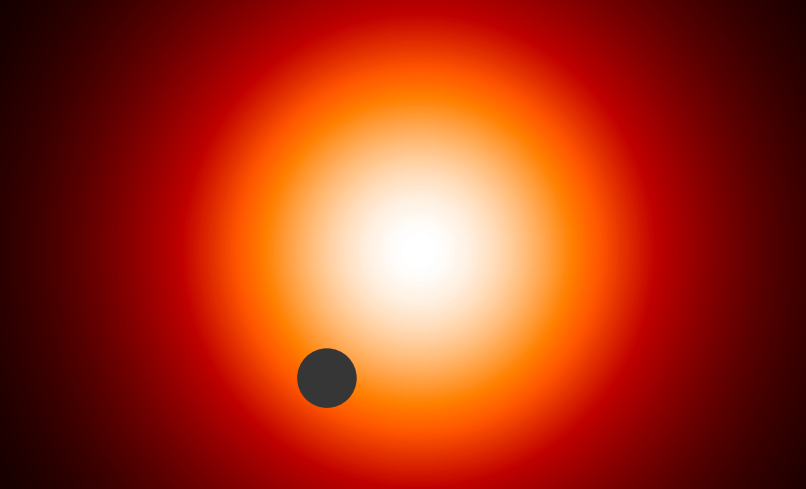
\includegraphics[width = 0.5\textwidth]{./images/WASP-43b-13.png}
    \caption{A realistic Python-simulated render of a transit of the WASP-43 system}
\end{figure}

\section{Target}

WASP-43 is a star in the Sextans constellation located at a distance of $284 \ \mathrm{ly}$ from Earth, with $m_{V} = 12.4$. It hosts one exoplanet, a Hot Jupiter known as WASP-43b \citep{Hellier_2011}. Notably, this system has the distinction of being the closest known planet to its host star. Table \ref{tab} lists the parameters for this system, along with which of them we assume and which we infer through our analysis.

\begin{table}[h]
    \centering
    \begin{tabular}{l|l|c}
    \hline
    \textbf{Parameter}   & \textbf{Known Value}    &        \textbf{Assumed/Inferred}                      \\
    \hline
    Mass of Star $(M_{\star}$) &   $ 0.72 \ \mathrm{M_{\odot}}$         &   Assumed        \\ \hline
    Radius of Star $(R_{\star})$ &      $ 0.68 \ \mathrm{R_{\odot}}$    &   Assumed        \\ \hline
    Limb Darkening &       $u_1 = 0.601$   &   Assumed      \\ 
    Coefficients &      $u_2 = 0.149$    &           \\ \hline
    Radius of Planet $(R_{p})$     &      $ 0.93 \ \mathrm{R_J}$        &   Inferred         \\   \hline
    Orbital Period $(T_{orb})$     &      $ 0.813 \ \mathrm{d}$          &   Inferred        \\     \hline
    Impact Parameter $(b)$    &      $ 0.66 $                          &   Inferred        \\  \hline
    Transit Depth & $ 28.9 \ \mathrm{mmag}$ & Inferred
    % Impact Parameter $(b)$    &      $ 0.698 \ \mathrm{d}$      \\ 
    
    \end{tabular}
    \caption{Summary of system parameters \citep{Hellier_2011}} \label{tab}
\end{table}


The quadratic limb darkening coefficients for WASP-43 were taken from \citet{Gillon_2012}, and have been used in our light curve model to accurately ascertain the brightness falloff of the star's surface. The impact parameter, $b$ is defined as the ratio of the apparent distance of the planet from the stellar centre to $R_{\star}$. It can be expressed in terms of semi-major axis $(a)$, inclination $(i)$ and $R_{\star}$.

\section{Observations}
We used the $0.7 m$ GROWTH-India Telescope \citep{Kumar_2022} to observe this target. Continuous observations of $60s$ each were made in the \textit{r'} band from $15{:}46$ to $16{:}29 \ \mathrm{UTC}$ on March 24th, 2023. The transit was predicted using the \href{https://astro.swarthmore.edu/transits/transits.cgi}{Swarthmore Transit Tracker} \citep{2013ascl.soft06007J}. We were able to get a few minutes baseline (pre-egress) data but could only observe till the transit midpoint due to a dome error halfway through the session.


\section{Photometry}

\begin{figure}[h]
    \centering
    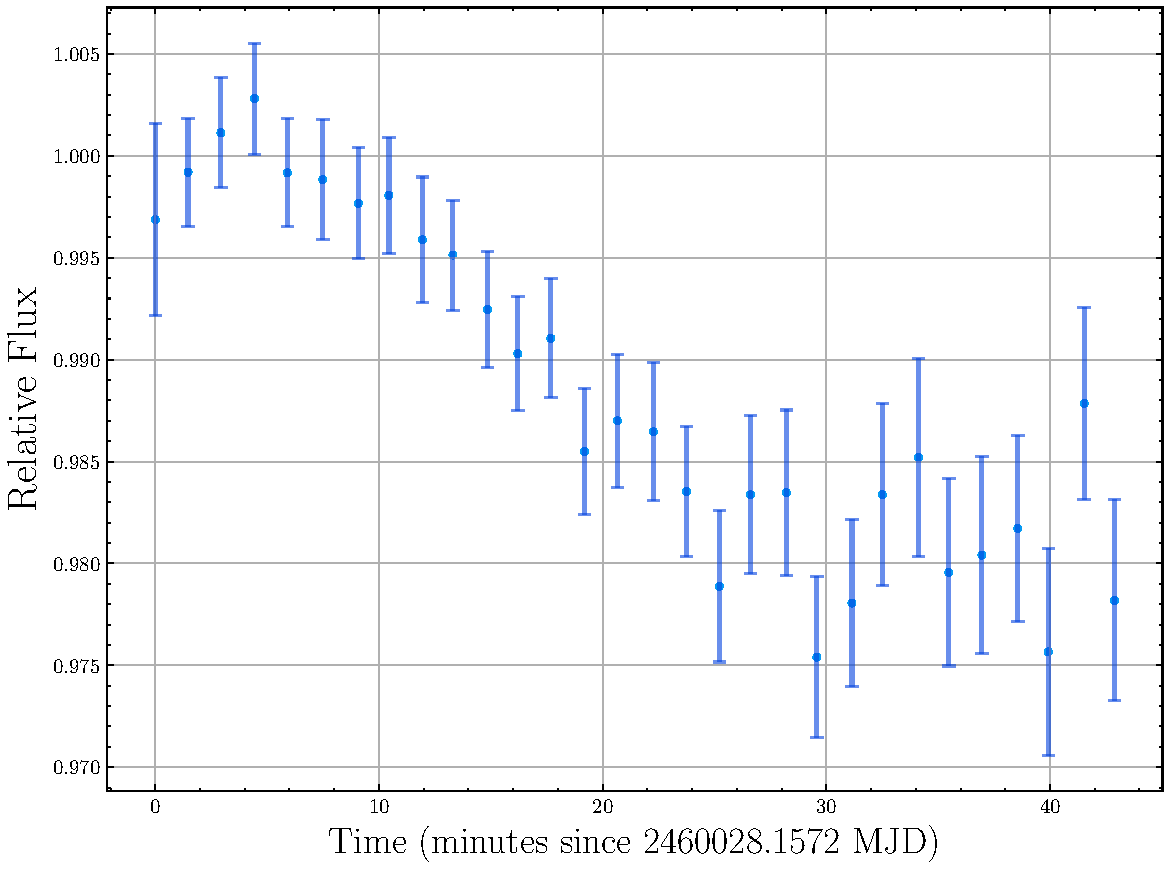
\includegraphics[width = 0.8\textwidth]{./images/raw.pdf}
    \caption{Raw normalised counts of WASP-43b transit}
    \label{raw}
\end{figure}

The 30 images obtained from the observations above were processed entirely in Python, using the \texttt{Astropy} \citep{astropy:2022} and \texttt{Photutils} \citep{larry_bradley_2022_6825092} Python packages. Since the brightness change is of the order of a few milli-magnitudes, regular aperture/PSF photometry is not usable due to large associated errors. Exoplanet data analysis thus utilises relative photometry, where the brightness of the target star is normalised against the variation of non-variable comparison stars available in the field to eliminate errors due to atmospheric conditions. 

We identified $6$ comparison stars in the field using the AAVSO Variable Star Plotter, and found the counts associated with the target and each of the comparison stars using a circular aperture. The flux of the target was then normalised as mentioned above, and offset to make the baseline $1.0$ and plotted in Figure \ref{raw}.

\section{Inference}
We next proceed to fit the obtained datapoints to a probabilistic transit model. This was done using a Python module, \texttt{exoplanet} \citep{exoplanet:joss}. This library utilises \texttt{PyMC3} \citep{exoplanet:pymc3}, which is a high-performance inference engine that utilises a variety of advanced Markov chain Monte Carlo (MCMC) methods to fit complex models with many parameters. It also makes use of \texttt{STARRY} \citep{exoplanet:luger18} for efficient computation of light curves for a given set of parameters. 

MCMC fitting methods rely on the user to supply an informed `guess' of the parameter space in the form of \textit{prior} probability distribution functions for each of the parameters that need to be inferred. These priors are then randomly and independently sampled and sequentially evolved on the basis of a \textit{likelihood} function which decides the accuracy of a parameter set. This is done by evaluating the model for the current set of parameters and comparing it to the observed data. The parameters are thus evolved over thousands of iterations, leading to empirical probability distribution functions (\textit{posteriors}) for the parameters, thus giving us the required estimates with error bounds.

\begin{table}[h]
    \centering
    \begin{tabular}{l|l}
    \hline
    \textbf{Parameter}   & \textbf{Prior}          \\
    \hline
    $R_p$   &       $\mathrm{Uniform}(0.06 ,0.12) \ \mathrm{R_J}$         \\ \hline
    $T_{orb}$   &       $ \exp{\left(\mathrm{Normal}(\mu = \log{0.9}, \sigma = 0.2)\right)} \ \mathrm{d} $     \\ \hline
    $T_{mid}$   &       $\mathrm{Normal}(\mu = 0.75, \sigma = 1) \ \mathrm{h}$         \\ \hline
    $b$   &       $\mathrm{Uniform}(0 ,1 + \mathrm{R_p/R_{\star}})$         \\ \hline

    % Impact Parameter $(b)$    &      $ 0.698 \ \mathrm{d}$      \\ 
    
    \end{tabular}
    \caption{Priors for the light curve model} \label{priors}
\end{table}

The free parameters in our case were $R_p$, $T_{orb}$, $b$ and $T_{mid}$, the mid-transit time. The priors for the variables are given in Table \ref{priors}. We tried to keep these sufficiently large and inclusive.

\begin{figure}[h]
    \centering
    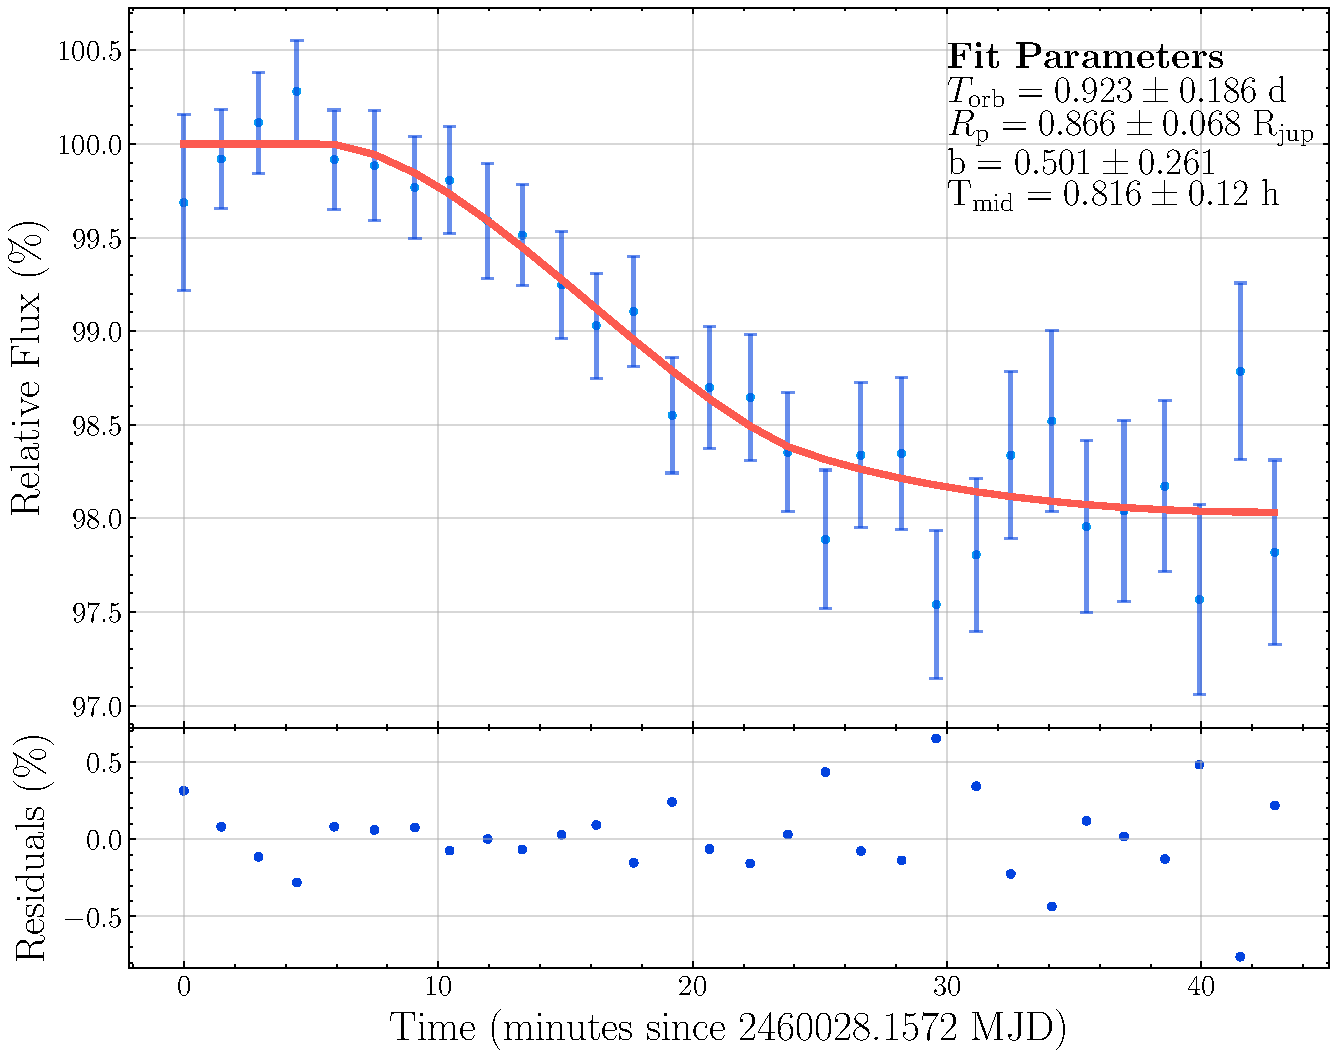
\includegraphics[width = 0.9\textwidth]{images/fit.pdf}
    \caption{WASP-43b Fitted Transit Light Curve}
    \label{fit}
\end{figure}

The fitted light curve along with parameters can be seen in Figure \ref{fit}. The obtained values have relatively large error bounds, and this is due to us having observed only the first half of the transit. The full posterior distribution can also be visualised as a corner plot \citep{corner} showing pairwise join distributions, as seen in Figure \ref{corner}.

\begin{figure}[h]
    \centering
    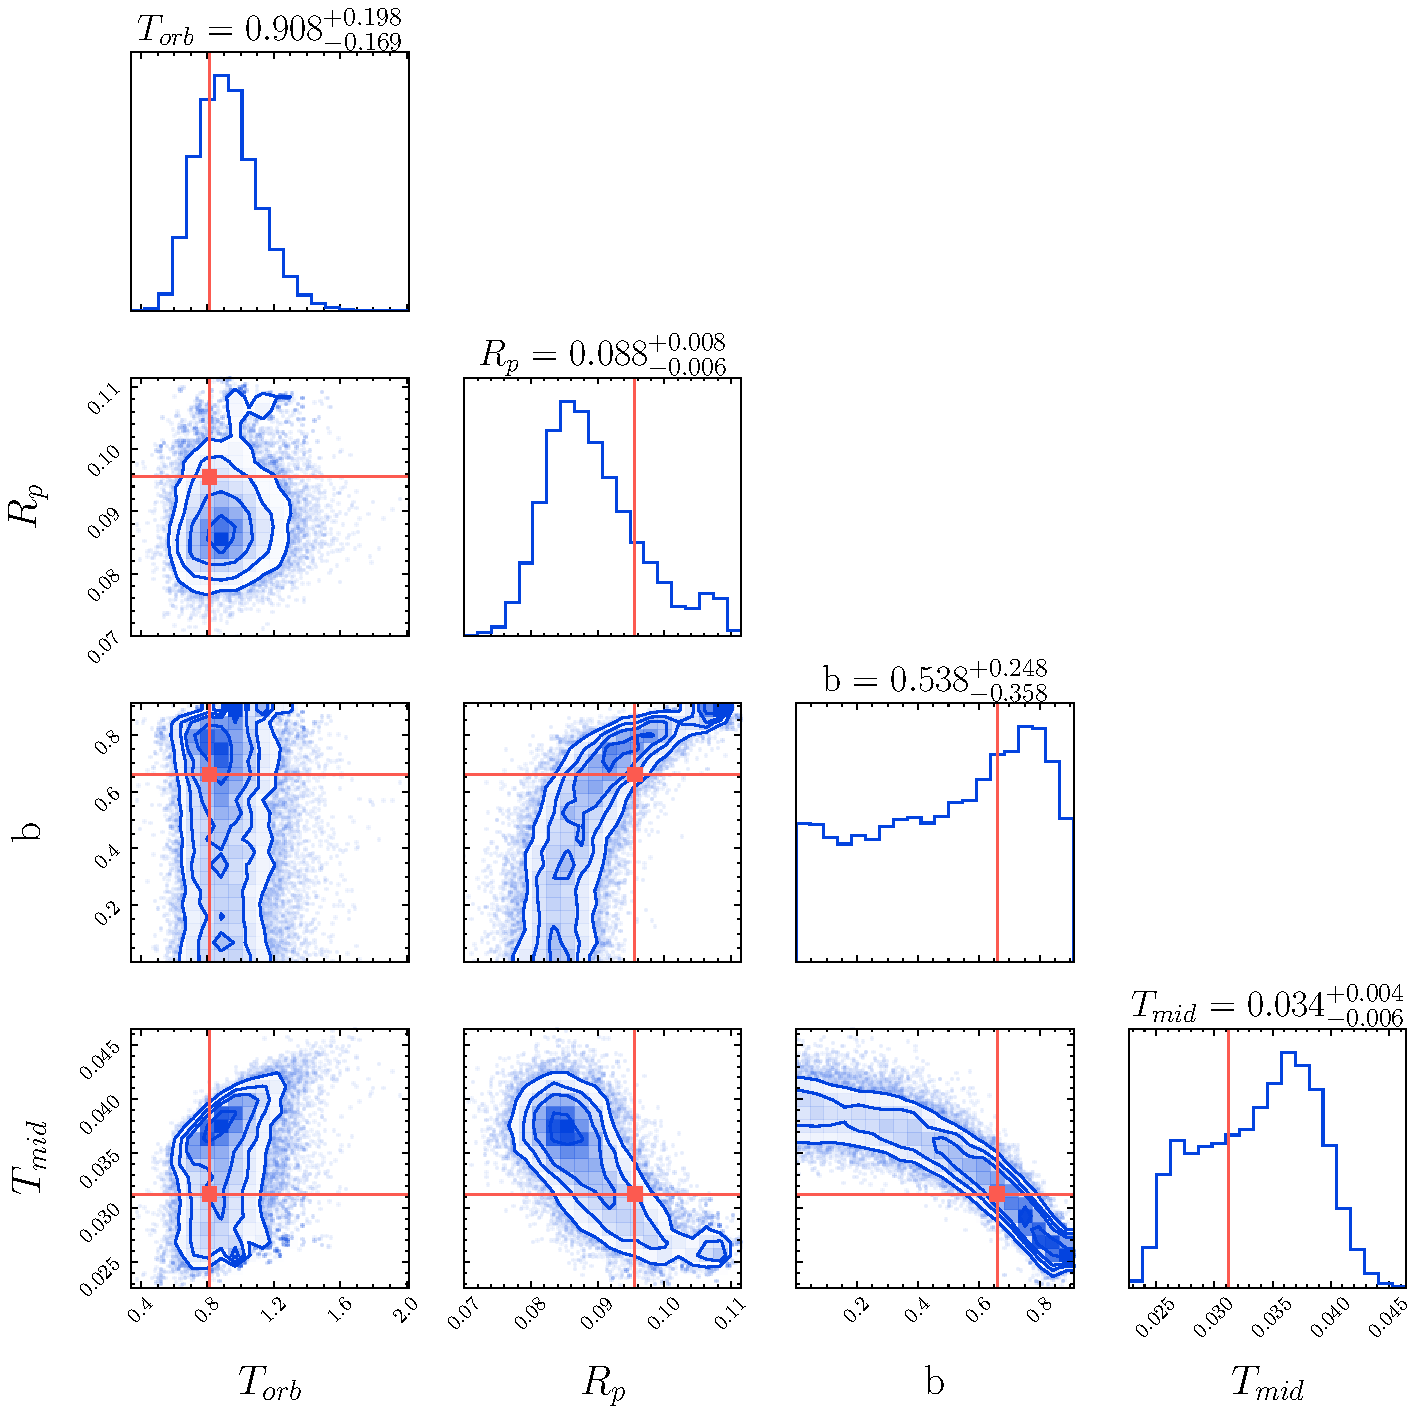
\includegraphics[width = 0.95\textwidth]{./images/corner.pdf}
    \caption{Joint distributions of parameter posteriors. The red lines mark true values.}
    \label{corner}
\end{figure}






\section{Results}
Table \ref{result} lists our results with $1\sigma$ error bounds and compares them to known values. As we could only observe half the transit, the error bars are quite large. But the known values are still within $1\sigma$ of the mean posterior value, which is a good indicator of the reliability of this method. In conclusion, GIT can be viably used for the confirmation or follow-up of smaller exoplanets using relative photometry and modern, efficient MCMC algorithms for inference.

\begin{table}[h]
    \centering
    \renewcommand{\arraystretch}{1.2}

    \begin{tabular}{l|l|l}
    \hline
    \textbf{Parameter}   & \textbf{Known Value}    &        \textbf{Inferred Value}                      \\ 
    \hline 
    Radius of Planet $(R_{p})$     &      $ 0.93 \ \mathrm{R_J}$        &   $0.856^{+0.077}_{-0.058} \ \mathrm{R_J} $        \\  \hline
    Orbital Period $(T_{orb})$     &      $ 0.813 \ \mathrm{d}$          &  $ 0.908^{+0.198}_{-0.169} \ \mathrm{d}$ \\    \hline
   Mid-transit time $(T_{mid})$    &      $ 45 \ \mathrm{min} $  &  $48.96^{+5.76}_{-8.64} \ \mathrm{min} $         \\  \hline 
   Impact Parameter $(b)$    &      $ 0.66 $                &   $0.538^{+0.248}_{-0.358}$  \\  
    % Impact Parameter $(b)$    &      $ 0.698 \ \mathrm{d}$      \\ 
    
    \end{tabular}
    \caption{Fitted parameters compared to known values from \cite{Hellier_2011}} 
    \label{result}
\end{table}


\newpage
\bibliographystyle{aasjournal}
\bibliography{references}

\end{document}
